\documentclass[]{article}
\usepackage[a4paper, total={5in,10in}]{geometry}
\usepackage{hyperref}
\usepackage{siunitx}
\usepackage{graphicx}
\usepackage{caption}
\usepackage[backend=biber]{biblatex}
\addbibresource{report.bib}

%opening
\title{EP2420 - Project 1: Task IV}
\author{André Silva}
\begin{document}

\maketitle

\section{\textbf{Task IV}}
\label{sec:1}

Since we are analysing \textit{VoD Flashcrowd}, we are going to convert our target values into an histogram of 31 labels, with midpoints 0, 1, 2, ..., 30.

\begin{figure}[h!]
    \centering
    \captionsetup{justification=centering}
    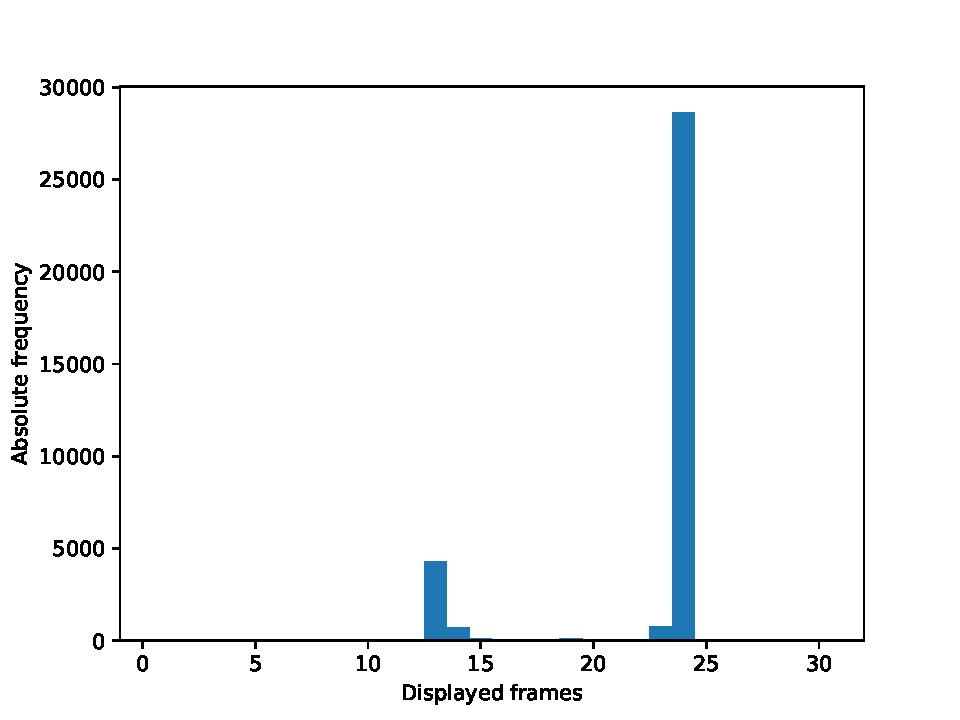
\includegraphics[width=0.72\textwidth,height=\textheight,keepaspectratio]{../result/project1/discretized_frames_hist.pdf}
    \caption{Histogram of the video frame rate on the interval $y\in[-0.5,30.5]$, with a bin size of 1}
    \label{fig:1}
\end{figure}

We then take each bin of the histogram as a class and fit a \textit{RandomForestClassifier}~\cite{RFC} to the data, which has been target of standardization by column and outlier removal.

The calculated \textsc{NMAE} for this model was approximatly $7.3\%$. In \textit{Task II}, we had been able to train a model which got $8.7\%$ \textsc{NMAE}, which was then marginally improved in \textit{Task III}. 

We can conclude by these results that the discretization of our target values allows us to better predict them. The loss of information as a result of this process is negligible, given the nature of the target values.

\pagebreak

\begin{figure}[h!]
    \centering
    \captionsetup{justification=centering}
    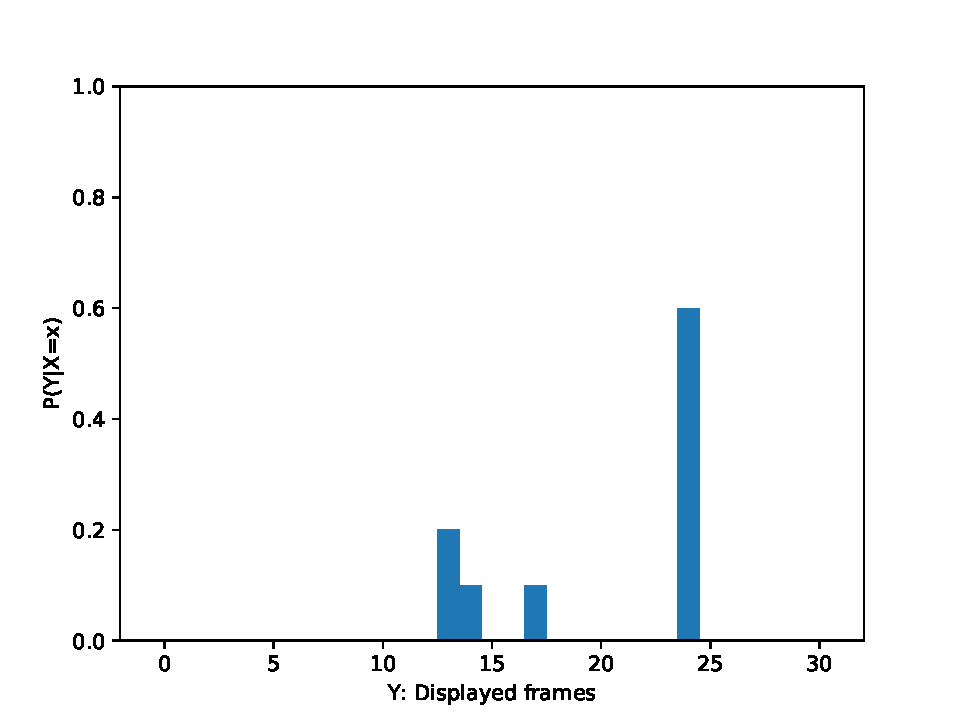
\includegraphics[width=0.72\textwidth,height=\textheight,keepaspectratio]{../result/project1/P(Y|X=x)_2643.pdf}
    \caption{Predicted histogram for a randomly selected sample of the test set. The measured target value was $24.0$}
    \label{fig:2}
\end{figure}

\begin{figure}[h!]
    \centering
    \captionsetup{justification=centering}
    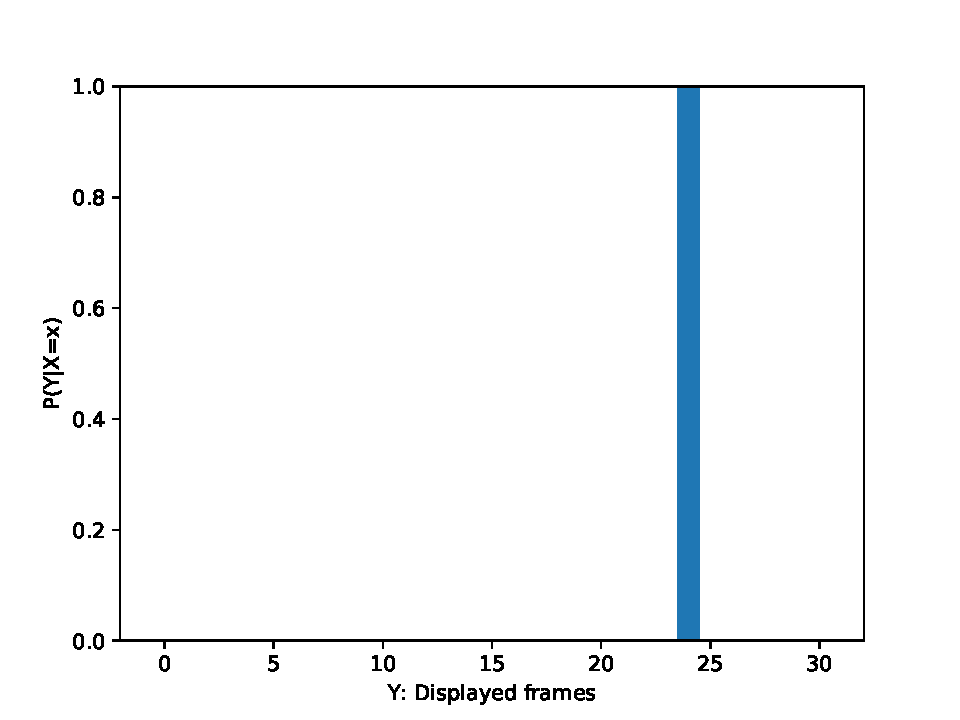
\includegraphics[width=0.72\textwidth,height=\textheight,keepaspectratio]{../result/project1/P(Y|X=x)_7272.pdf}
    \caption{Predicted histogram for a randomly selected sample of the test set. The measured target value was $24.0$}
    \label{fig:3}
\end{figure}

In Figures \ref{fig:2} and \ref{fig:3}, we can see the predicted histograms for two randomly selected samples of the test set, both with a measured value of $24.0$.

In the first case, $P(Y|X)$ is distributed between four classes, 13, 14, 17 and 24, whereas in the second case it is concentrated entirely on class 24. 
We can extract from this that, when the system is in a state equivalent to the first sample, it is more unstable relative to the second, and that we can expect some disturbances in the video frame rate registered by the client.

\printbibliography

\end{document}
